\documentclass[aspectratio=169,11pt]{beamer}

\usepackage{tikz}
\usepackage[utf8]{inputenc}
\usepackage[T1]{fontenc}
\usepackage{lmodern}
\usepackage{amsmath, amssymb, bm}
\usepackage{booktabs}
\usepackage{graphicx}
\usepackage{listings}
\usefonttheme{professionalfonts}

\definecolor{main}{RGB}{25,25,25}
\definecolor{accent}{RGB}{0,95,160}
\definecolor{accent2}{RGB}{220,120,40}

\setbeamercolor{normal text}{fg=main}
\setbeamercolor{structure}{fg=accent}
\setbeamercolor{frametitle}{fg=main,bg=white}
\setbeamercolor{title}{fg=main}
\setbeamercolor{block title}{fg=white,bg=accent}
\setbeamercolor{block body}{fg=main,bg=white}
\setbeamercolor{block title example}{fg=white,bg=accent2}
\setbeamercolor{block body example}{fg=main,bg=white}

\setbeamertemplate{navigation symbols}{}

\setbeamertemplate{headline}{
  \leavevmode
    \begin{beamercolorbox}[wd=.995\paperwidth,ht=0.1cm,dp=0.05cm]{structure}
    \hspace{0.1cm}
    \textcolor{white}{\insertsection}
    \end{beamercolorbox}
}

\setbeamertemplate{footline}{
\leavevmode%
\hbox{%
\begin{beamercolorbox}[wd=.49\paperwidth,ht=2.5ex,dp=1.2ex,left]{title in head/foot}%
\end{beamercolorbox}%
\begin{beamercolorbox}[wd=.49\paperwidth,ht=2.5ex,dp=1.2ex,right]{author in head/foot}%
\insertframenumber/\inserttotalframenumber\hspace{0.3em}
\end{beamercolorbox}%
}
\vskip0pt
}

\setbeamertemplate{frametitle}{
  \vspace{0.3cm}
  \insertframetitle
  \par
  \color{accent}\rule{\linewidth}{0.6pt}
}

\lstdefinestyle{rcode}{
  language=R,
  basicstyle=\ttfamily\scriptsize,
  keywordstyle=\color{accent}\bfseries,
  commentstyle=\color{gray},
  stringstyle=\color{accent2},
  showstringspaces=false,
  columns=fullflexible,
  keepspaces=true,
  frame=single,
  rulecolor=\color{accent},
  framerule=0.4pt,
  xleftmargin=0.2cm,
  xrightmargin=0.2cm
}

\title[Bayesian Fraud Detection]{Bayesian Fraud Detection}
\subtitle{From Prior Knowledge to Posterior Uncertainty}
\author{Giovanni La Gioia}
\newcommand{\faculty}{USI - Faculty of Informatics}
\newcommand{\course}{Introduction to Bayesian Learning}
\date{4th June 2026}

\begin{document}

\begin{frame}
  \titlepage

  \begin{center}
  \small
  \textbf{\faculty}\\
  \textbf{\course}
  \end{center}
\end{frame}

\section{Introduction}

\begin{frame}{Context}

\begin{itemize}
  \item Modern financial systems generate high-volume transactional data with complex temporal patterns.
  \item Anomaly detection aims to identify rare or unusual transactions that deviate from normal behaviour.
  \item In real-world settings, true fraud labels are often unavailable or incomplete.
  \item This motivates the use of unsupervised methods and probabilistic models to estimate anomaly risk.
  \item Transaction-level anomaly detection is inherently a \textbf{rare event classification problem}, where class imbalance and uncertainty are central challenges.
\end{itemize}

\end{frame}

\begin{frame}{Objective}

\begin{block}{Motivation}

\begin{columns}
\column{0.55\textwidth}

\begin{itemize}
  \item Detect anomalous transactions without having true fraud labels.
  \item Use Isolation Forest to construct a proxy anomaly label.
  \item Show how Bayesian inference models uncertainty, not only point estimates.
\end{itemize}

\column{0.45\textwidth}
\centering
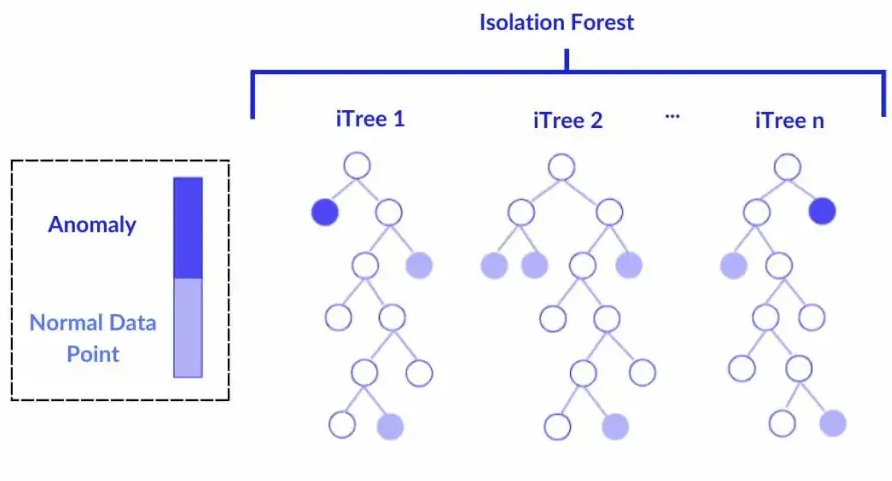
\includegraphics[width=\textwidth]{illustration-isolation-forest.png}

\end{columns}
\end{block}

\end{frame}

\section{Bayesian Inference}

\begin{frame}{Bayesian Starting Point}
  \begin{block}{Bayes' rule}
  \[
  p(\theta \mid y)
  =
  \frac{p(\theta)\,p(y \mid \theta)}{p(y)}
  \]

    \[
    \text{posterior}
    =
    \frac{\text{prior} \times \text{likelihood}}{\text{marginal likelihood}}
    \]
  \end{block}

  \vspace{0.15cm}

  \begin{center}
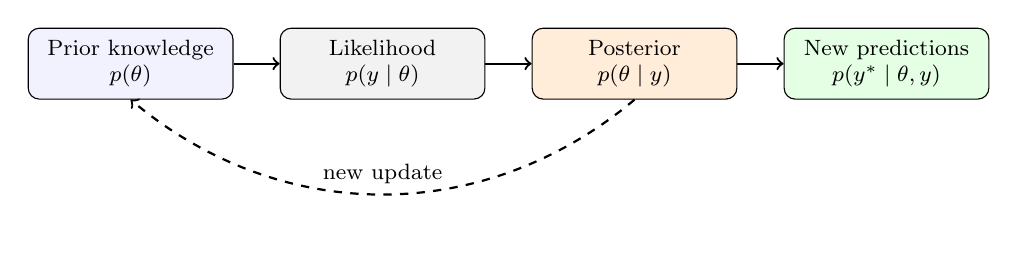
\begin{tikzpicture}[
  every node/.style={font=\footnotesize, align=center},
  box/.style={draw, rounded corners, minimum width=2.6cm, minimum height=0.9cm, fill=blue!5},
  arrow/.style={->, thick}
]

\node[box] (prior) at (0,0) {Prior knowledge\\$p(\theta)$};

\node[box, fill=gray!10] (data) at (3.2,0) {Likelihood\\$p(y \mid \theta)$};

\node[box, fill=orange!15] (post) at (6.4,0) {Posterior\\$p(\theta \mid y)$};

\node[box, fill=green!10] (pred) at (9.6,0) {New predictions\\$p(y^\ast \mid \theta, y)$};

\draw[arrow] (prior) -- (data);
\draw[arrow] (data) -- (post);
\draw[arrow] (post) -- (pred);

% LOOP BACK
\draw[arrow, dashed] (post.south) to[bend left=40] node[above] {new update} (prior.south);

\end{tikzpicture}
\end{center}

\end{frame}

\begin{frame}{What Each Term Means}
  \begin{block}{Components}
  \begin{itemize}
    \item \textbf{Prior}: what we believe before observing the current data.
    \item \textbf{Likelihood}: how compatible the data are with each parameter value.
    \item \textbf{Posterior}: updated belief after observing the data.
    \item \textbf{Marginal likelihood}: normalization constant.
  \end{itemize}
  \end{block}

  \begin{exampleblock}{Marginal likelihood}
  \[
  p(y)=\int p(\tilde{\theta})\,p(y \mid \tilde{\theta})\,d\tilde{\theta}
  \]
  \end{exampleblock}
\end{frame}

\begin{frame}{Why the Marginal Matters}
  \begin{block}{Conjugate models (from the course)}
  \begin{itemize}
    \item \textbf{Beta--Binomial:} closed-form posterior for Bernoulli data.
    \item \textbf{Gaussian--Gaussian:} conjugate update for mean estimation with known variance.
    \item In both cases, the posterior is available analytically thanks to conjugacy.
  \end{itemize}
  \end{block}

  \begin{block}{General case}
  \begin{itemize}
    \item In more realistic models, the integral is not available in closed form.
    \item This motivates simulation-based inference (MCMC) to obtain posterior distribution of $\theta$
  \end{itemize}
  \end{block}
   \vspace{-0.3cm}

  \[
  p(\theta \mid y) \propto p(\theta)\,p(y \mid \theta)
  \]
\end{frame}

\begin{frame}{Workflow}
  \begin{block}{Project presentation path}
  \begin{enumerate}
    \item Data cleaning and feature engineering.
    \item Build anomaly labels with Isolation Forest algorithm.
    \item Start with a Beta-Binomial model for the global anomaly rate.
    \item Track sequential posterior uncertainty over time.
    \item Move to Bayesian logistic regression with transaction features.
    \item Use MCMC for the posterior that cannot be obtained analytically.
    \item Obtain metrics and uncertainty estimates for predictions on the test set.
  \end{enumerate}
  \end{block}
\end{frame}

\section{Data and Labels}

\begin{frame}{Dataset Overview}
      \begin{itemize}
        \item Anonymous bank transaction record dataset from 2017 to 2019.
        \item $116201$ transactions in total.
        \item Dataset features: transaction date, withdrawal amount, deposit amount, cheque number, and account balance.
        \item Irrelevant variables (e.g. cheque number and textual descriptions) were removed and some features were engineered (e.g. log time, balance amount ratio).
      \end{itemize}
\end{frame}

\begin{frame}{Anomaly Label Construction}
  \begin{columns}
    \begin{column}{0.48\textwidth}
      \begin{itemize}
        \item True fraud labels are not available.
        \item Isolation Forest assigns an anomaly score.
        \item Transactions above the 95\% quantile are labeled as anomalies.
        \item Therefore, the 5\% anomaly rate is fixed by construction.
      \end{itemize}
    \end{column}
    \begin{column}{0.52\textwidth}
      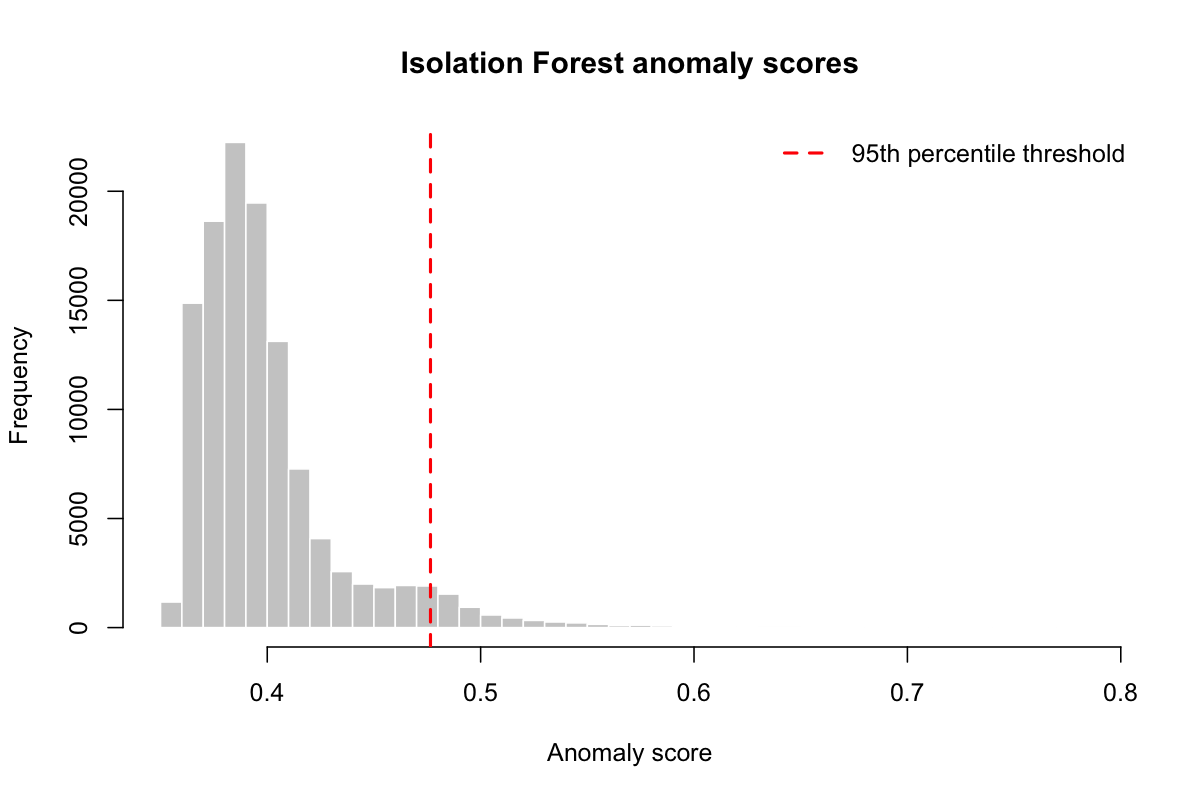
\includegraphics[width=\textwidth]{../plots/01_isolation_forest_scores.png}
    \end{column}
  \end{columns}
\end{frame}

\begin{frame}[fragile]{Code: Anomaly Label}
\begin{block}{Isolation Forest thresholding}
\begin{lstlisting}[style=rcode]
X <- data[, c("amount", "log_time", "balance",
              "is_withdrawal", "balance_amount_ratio",
              "weekday")]

model <- isolation.forest(X, seed = 123, nthreads = 1)
score <- predict(model, X)

threshold <- quantile(score, 0.95, na.rm = TRUE)
data$Y <- ifelse(score > threshold, 1, 0)
\end{lstlisting}
\end{block}

\end{frame}

\section{Analytical Posterior}

\begin{frame}{Beta-Binomial Model}
  \begin{block}{Modeling precondition}
  \begin{itemize}
    \item The 5\% anomaly rate is a modeling precondition, as prior information.
    \item The first Bayesian model tests how this prior interacts with a random subsample.
  \end{itemize}

  \[
  Y_i \sim \text{Bernoulli}(\pi),
  \qquad
  \pi \sim \text{Beta}(\alpha_0,\beta_0)
  \]
  \end{block}
  \begin{block}{Closed-form update}
  \[
  \pi \mid Y
  \sim
  \text{Beta}(\alpha_0+k,\ \beta_0+n-k)
  \]
  \end{block}
  \begin{itemize}
    \item $k$: number of observed anomalies; $n$: number of sampled transactions.
    \item Conjugacy gives a closed-form posterior.
  \end{itemize}
\end{frame}

\begin{frame}{Posterior Under Different Priors}
  \begin{columns}
    \begin{column}{0.42\textwidth}
      \begin{itemize}
        \item Random subsample: 250 transactions.
        \item Observed anomalies: 13.
        \item Informative priors pull the posterior toward 5\%.
        \item Stronger priors reduce posterior uncertainty.
      \end{itemize}
    \end{column}
    \begin{column}{0.58\textwidth}
      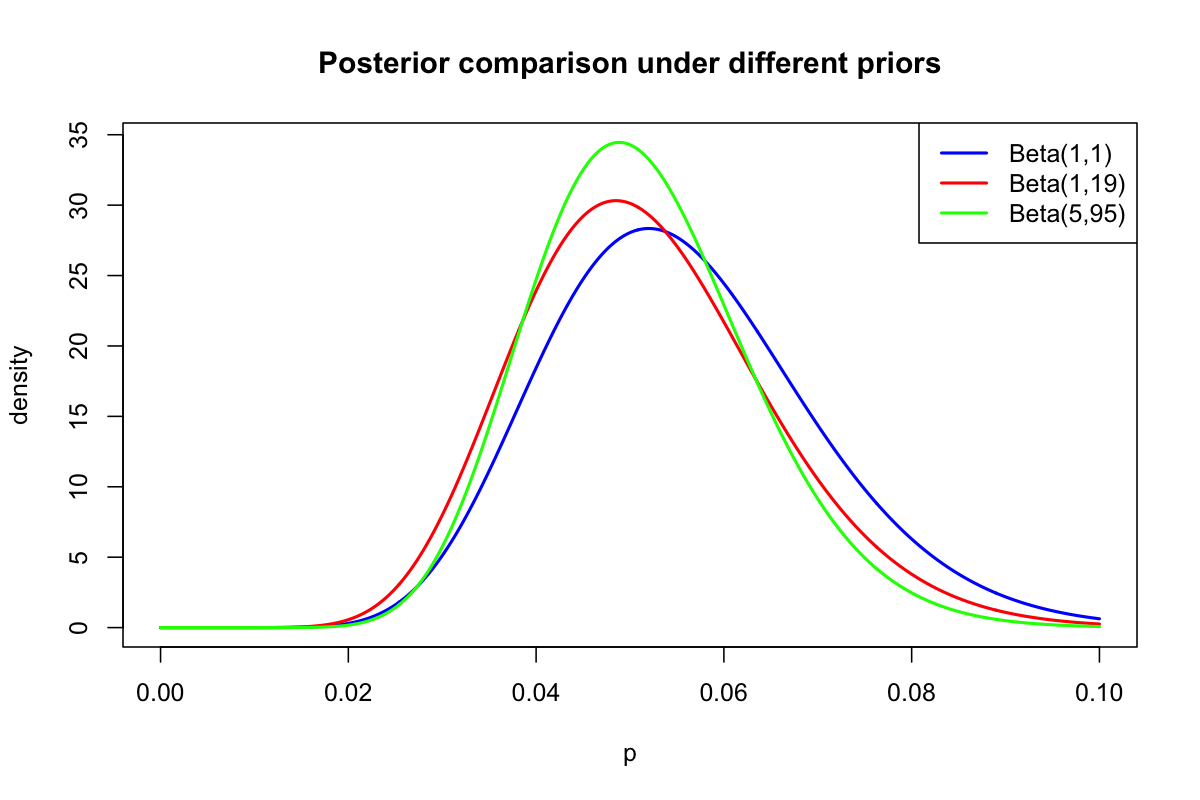
\includegraphics[width=\textwidth]{../plots/02_beta_posterior_comparison.png}
    \end{column}
  \end{columns}
\end{frame}

\section{Sequential Learning}

\begin{frame}{Sequential Bayesian Learning}
  \begin{block}{Online update}
  \[
  \alpha_t=\alpha_0+k_t,
  \qquad
  \beta_t=\beta_0+t-k_t
  \]

  \[
  \mathbb{E}[\pi_t \mid Y_t]
  =
  \frac{\alpha_t}{\alpha_t+\beta_t}
  \]
  \end{block}

  \begin{itemize}
    \item Here $\alpha_0,\beta_0$ represent a non-informative prior.
    \item As more transactions are observed, uncertainty decreases.
  \end{itemize}
\end{frame}

\begin{frame}{Anomaly Rate Over Time}
  \begin{columns}
    \begin{column}{0.38\textwidth}
      \begin{itemize}
        \item Final posterior mean: $\mathbf{E}[\pi \mid Y] = 0.050007$.
        \item Final 95\% credible interval for $\pi$ variable: $[0.048960,\ 0.051063]$.
        \item The interval becomes very narrow with the full sequence.
      \end{itemize}
    \end{column}
    \begin{column}{0.62\textwidth}
      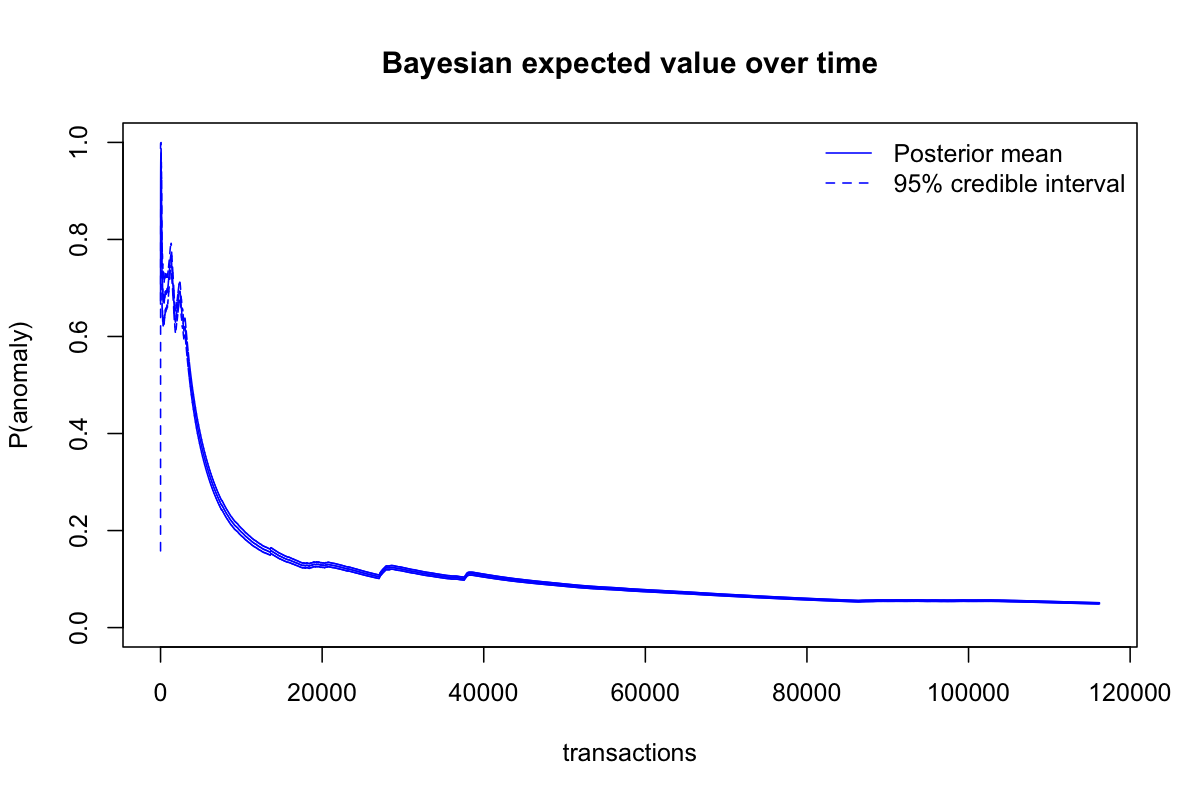
\includegraphics[width=\textwidth]{../plots/03_sequential_bayesian_learning.png}
    \end{column}
  \end{columns}
\end{frame}

\section{MCMC Estimation}

\begin{frame}{Why Move Beyond Beta-Binomial?}
  \begin{block}{Limitation of the global model}
  \begin{itemize}
    \item Beta-Binomial estimates only global anomaly probability.
    \item It does not use transaction-level information, so no interpretability.
    \item Fraud risk should vary across transactions.
    \item Considering $Y_i \sim \text{Bernoulli}(\pi_i)$ with $Y_i$ as anomaly indicator and $\pi_i$ as the transaction anomaly probability:
  \end{itemize}
  \end{block}

  \[
  \text{logit}(\pi_i)
  =
  \log \frac{\pi_i}{1-\pi_i}
  =
  \beta_0+\sum_{j=1}^{p}\beta_j x_{ij}
  \]
\end{frame}

\begin{frame}{Why MCMC?}
  \begin{block}{Non-conjugate posterior}
  \begin{itemize}
    \item Logistic regression has a non-conjugate likelihood.
    \item The posterior cannot be derived analytically.
    \item The marginal likelihood requires an intractable integral.
  \end{itemize}
  \end{block}

  \[
  p(\bm{\beta}\mid Y,X)
  =
  \frac{p(\bm{\beta})p(Y\mid X,\bm{\beta})}
  {\int p(\bm{\beta})p(Y\mid X,\bm{\beta})d\bm{\beta}}
  \]
\end{frame}

\begin{frame}{MCMC Intuition}
  \begin{block}{Simulation from the posterior}
  \[
  \bm{\beta}^{(1)},\bm{\beta}^{(2)},\ldots,\bm{\beta}^{(S)}
  \sim
  p(\bm{\beta}\mid Y,X)
  \]
  \end{block}

  \begin{itemize}
    \item MCMC samples plausible parameter configurations.
    \item Predictions average over many sampled models.
    \item This gives both posterior mean predictions and credible intervals.
  \end{itemize}
\end{frame}

\begin{frame}[fragile]{Code: Bayesian Logistic Regression}
\begin{block}{MCMC fit with \texttt{brms} with Cauchy prior}
\begin{lstlisting}[style=rcode]
bayes_formula <- Y ~ amount + balance + log_time +
  is_withdrawal + balance_amount_ratio + weekday

fit_bayes <- brm(
  bayes_formula,
  family = bernoulli(link = "logit"),
  data = train,
  prior = c(prior(cauchy(0, 2.5), class = "b"),
            prior(cauchy(0, 2.5), class = "Intercept")),
  chains = 4, iter = 1200, warmup = 600,
  seed = 123
)
\end{lstlisting}
\end{block}
\end{frame}

\section{Results}
\begin{frame}{Bayesian Logistic Regression Results with Cauchy Prior}

\begin{block}{Model specification}
\begin{itemize}
  \item Prior: $\text{Cauchy}(0,2.5)$ (weakly informative)
  \item 92,960 training observations, 2,400 posterior draws
\end{itemize}
\end{block}

\begin{block}{Key feature effects (log-odds scale)}
\begin{itemize}
  \item \textbf{balance amount ratio (-22.26):} strongest effect; high imbalance strongly indicates anomalies.
  \item \textbf{log time (-1.84):} later transactions are less likely to be anomalous.
  \item \textbf{Sunday (+5.57):} extremely high anomaly concentration on Sundays.
  \item \textbf{is\_withdrawal (+0.34):} withdrawals slightly more suspicious than deposits.
\end{itemize}
\end{block}
\end{frame}

\begin{frame}{MCMC Diagnostics and Convergence}
  \begin{table}
    \centering
    \small
    \begin{tabular}{lrrr}
      \toprule
      \textbf{Prior} & \textbf{Max $\hat{R}$} & \textbf{Min bulk ESS} & \textbf{Min tail ESS} \\
      \midrule
      Normal(0,1) & 1.003 & 1045.7 & 1251 \\
      Normal(0,2) & 1.005 & 831.1 & 1318 \\
      Cauchy(0,2.5) & 1.003 & 807.8 & 1150 \\
      \bottomrule
    \end{tabular}
  \end{table}

  \begin{itemize}
    \item $\hat{R}\approx 1$ indicates that the different chains are mixing well and converge to the same posterior distribution.
    \item Effective sample sizes are sufficient for fixed effects.
  \end{itemize}
\end{frame}

\begin{frame}{Classification Metrics}

\begin{block}{Confusion matrix quantities}
\[
\begin{array}{cc}
TP=\text{true positives} & TN=\text{true negatives} \\
FP=\text{false positives} & FN=\text{false negatives}
\end{array}
\]
\end{block}

\begin{block}{Metric definitions}
\[
\text{Sensitivity}=\text{Recall}=\frac{TP}{TP+FN}
\]
\[
\text{Specificity}=\frac{TN}{TN+FP}
\]
\[
\text{Precision}=\frac{TP}{TP+FP}
\]
\end{block}

\end{frame}

\begin{frame}{Predictive Performance}

\begin{table}
\centering
\small
\begin{tabular}{lrrrrr}
\toprule
\textbf{Model} & \textbf{Threshold} & \textbf{AUC} & \textbf{Recall} & \textbf{Precision} & \textbf{F1} \\
\midrule
Frequentist & 0.50 & 0.9313 & 0.4707 & 0.7822 & 0.5877 \\
Bayes N(0,1) & 0.50 & 0.9767 & 0.6103 & 0.7919 & 0.6894 \\
Bayes N(0,2) & 0.50 & 0.9781 & 0.6164 & 0.7874 & 0.6915 \\
Bayes Cauchy & 0.50 & 0.9790 & 0.6198 & 0.7849 & 0.6927 \\
Cauchy (opt.) & 0.1493 & 0.9790 & 0.9172 & 0.5872 & 0.7160 \\
\bottomrule
\end{tabular}
\end{table}

\vspace{0.1cm}

\begin{block}{Key insights}

\begin{itemize}
  \item Bayesian models consistently improve metrics performance.
  \item Lower optimal threshold significantly increases recall, reducing missed anomalies (false negatives) that would otherwise go undetected.
  \item This improvement comes at the cost of lower precision due to more false positives.
\end{itemize}

\end{block}
\end{frame}

\begin{frame}{ROC Comparison}
  \centering
  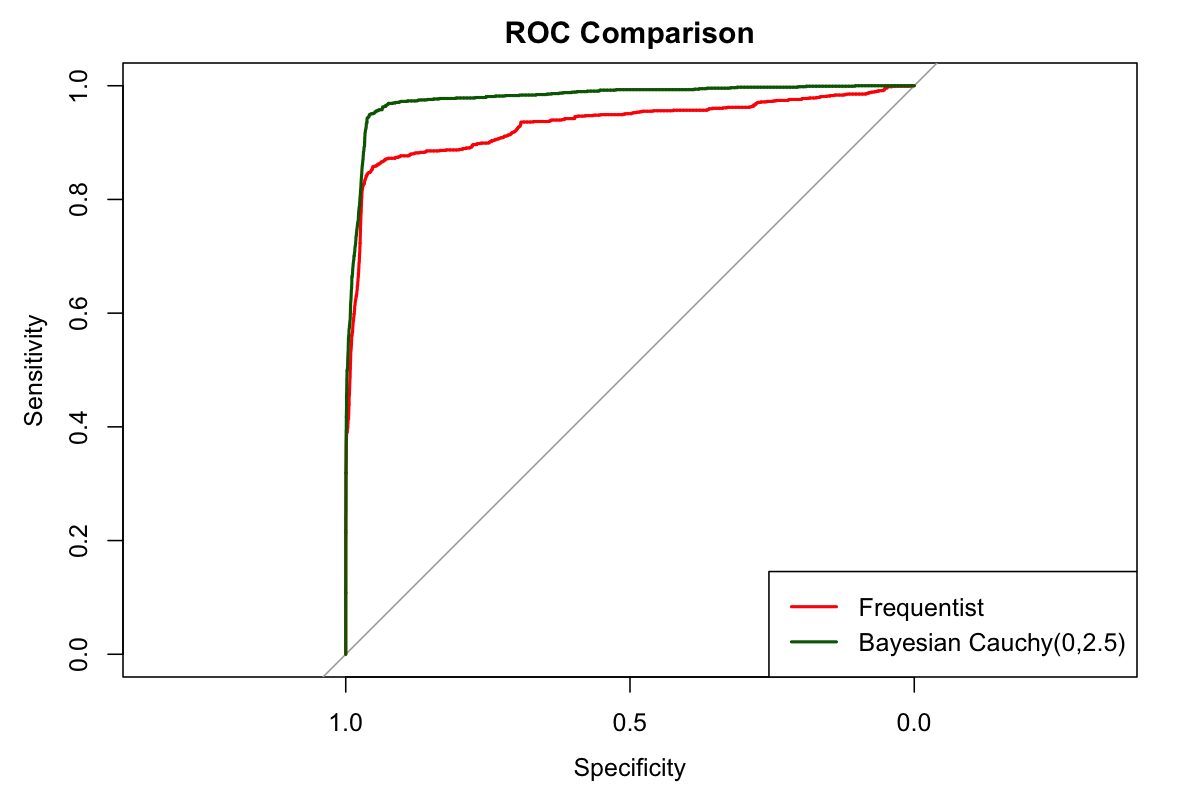
\includegraphics[height=0.78\textheight]{../plots/04_roc_comparison.png}
\end{frame}

\begin{frame}{Posterior Predictive Uncertainty}
  \begin{columns}
    \begin{column}{0.37\textwidth}
      \begin{itemize}
        \item Each prediction is a distribution.
        \item Credible intervals flag uncertain cases.
        \item This is useful for manual review and risk scoring.
      \end{itemize}
    \end{column}
    \begin{column}{0.63\textwidth}
      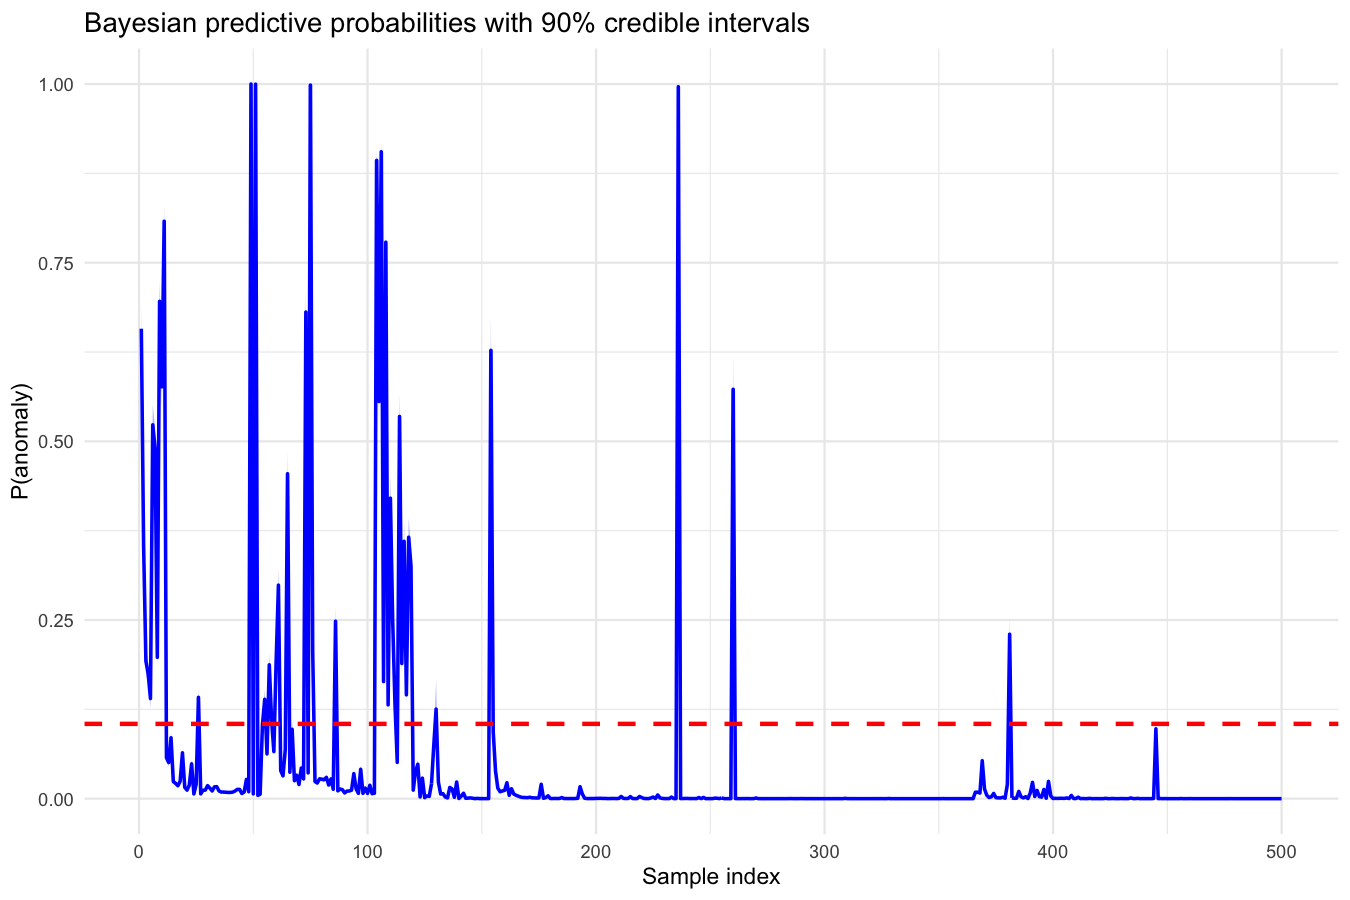
\includegraphics[width=\textwidth]{../plots/05_bayesian_predictive_uncertainty.png}
    \end{column}
  \end{columns}
\end{frame}

\section{Conclusion}

\begin{frame}{Takeaways \& Limitations}
  \begin{block}{Summary}
  \begin{itemize}
    \item Bayesian inference turns assumptions and data into posterior distributions.
    \item MCMC is needed when the marginal integral is not analytically available.
    \item Bayesian logistic regression gives competitive predictions and uncertainty.
  \end{itemize}
  \end{block}

  \begin{block}{Main limits}
  \begin{itemize}
    \item The target is an Isolation Forest proxy label, not confirmed fraud.
    \item Performance measures consistency with the labeling rule.
    \item A production setting would require temporal validation and true fraud outcomes.
  \end{itemize}
  \end{block}
  \end{frame}

\begin{frame}{References}

\large

\textit{Liu, F. T., Ting, K. M., and Zhou, Z.-H. (2008). Isolation Forest.}
\vspace{0.2cm}

\textit{Gelman, A., Jakulin, A., Pittau, M. G., and Su, Y.-S. (2008). A weakly informative default prior distribution for logistic and other regression models.}
\vspace{0.2cm}

\textit{Watsky, A. \href{https://www.kaggle.com/datasets/apoorvwatsky/bank-transaction-data}{Extracted bank account statements of various bank accounts}.}
\vspace{0.2cm}

\textbf{Repository}: \href{https://github.com/giolagioia/Bayes-Anomaly-Detection}{github.com/giolagioia/Bayes-Anomaly-Detection}

\end{frame}

\end{document}
